\section{Exercise 1}
\label{sec:exercise1}

The first exercise's objective is to take a grasp's Metasploit's \texttt{auxiliary} library and to use it for some simple reconnaissance tasks on the network.

Metasploit is packed with a deep auxiliary library, called the Metasploit \textit{EXploitation} library (and known as \texttt{lib}\texttt{/msf}\texttt{/core} within the Ruby source code). Its objective is to automate as much as possible typical reconnaissance tasks.

The auxiliary library provides a lot of tools. They include server capture modules (for sniffing credentials or collecting password hashes), scanners (of all sorts: TCP, UDP, HTTP, etc...), and administrative modules (for directory listing, identification of admin panels, and more), fuzzers, brute forcers, and even DoS managers.

\subsection{TCP scanning}
\label{sec:exercise1:tcpscanning}

Let us start by examining open some ports on our targets. We can either use \texttt{Nmap} or one of the auxiliary Metasploit modules. We'll defer the use of the former to the next exercise, which will also employ Metasploit's database. For now, let's load the TCP scanner module and run it against the whole subnet.\cite{online:msf-scanning-enumeration}\cite{online:msf-auxmodules}

\begin{lstlisting}
use auxiliary/scanner/portscan/tcp
\end{lstlisting}

\begin{figure}[htbp]
	\centering
	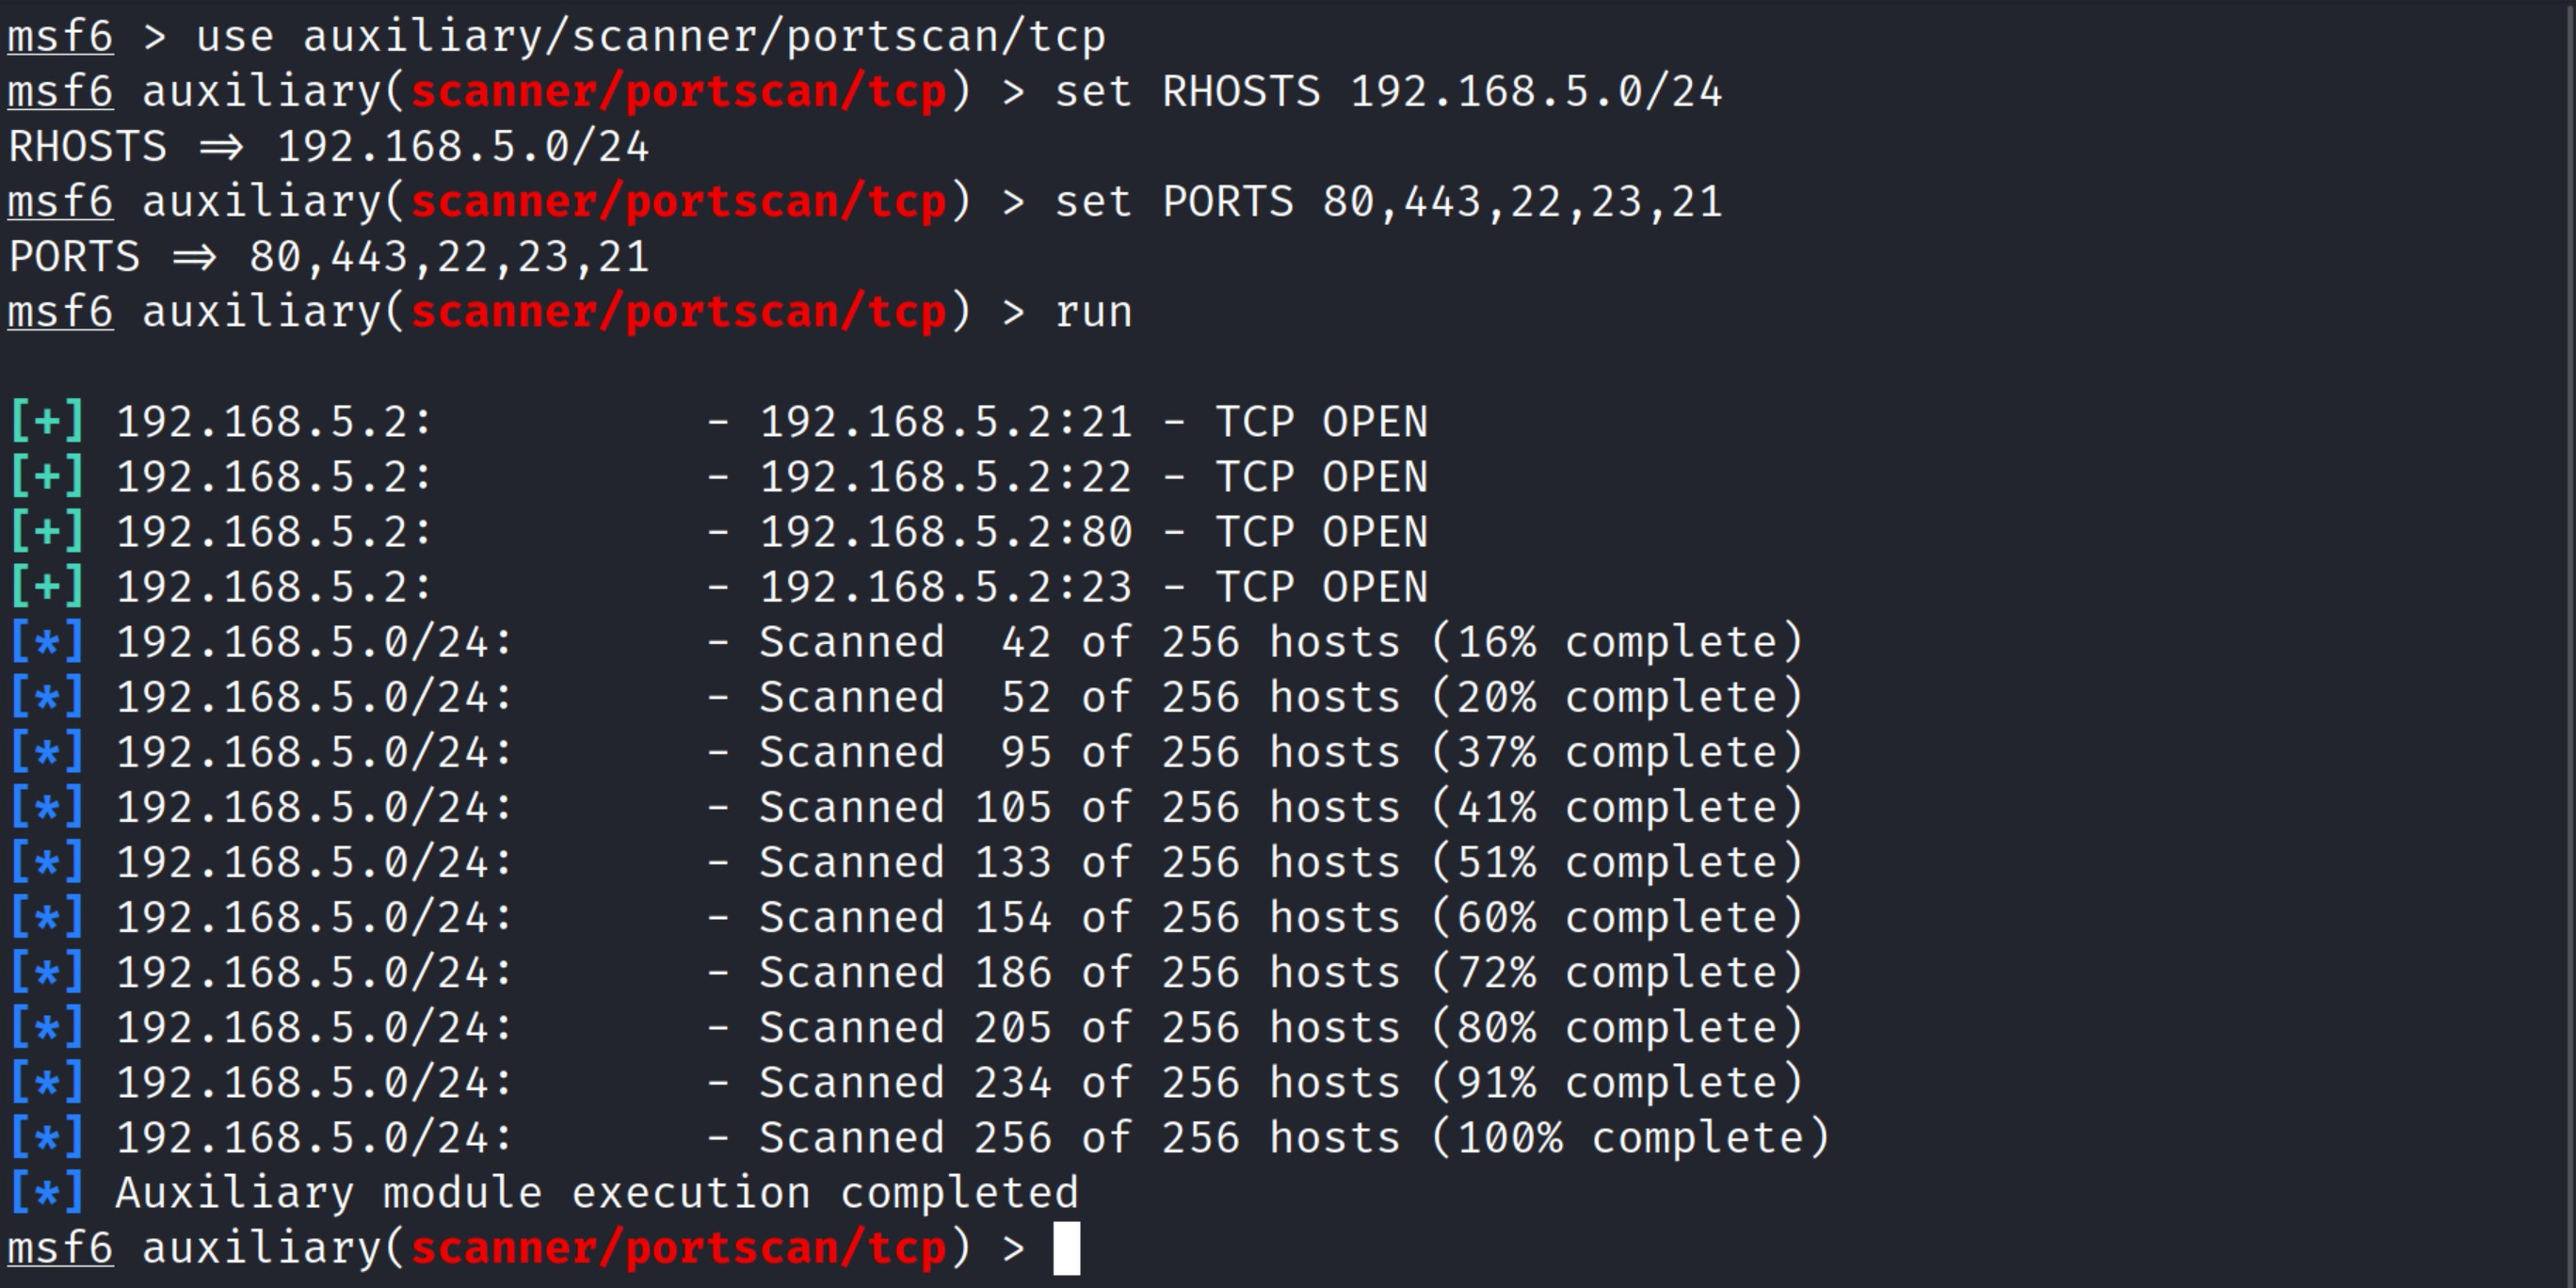
\includegraphics[width=0.9\textwidth]{../drawable/exercise_1_screenshots/es1-scan.jpg}
	\caption{Setting options for the \texttt{TCP} scanner and running it}
	\label{fig:ex1:scan}
\end{figure}

Metasploit still provides various scanners, such as a \texttt{SYN} one. Additionally, we deliberately inserted a few ports in this example just to showcase the usage of the tool. In Section \ref{sec:ex2} a more accurate and complete scan will be executed.

\subsection{SSH scanning and brute forcing}

Next, we show an example of \texttt{SSH} server scanning and brute forcing. We just verified with the TCP scanner that the Metasploitable machine is exposing an \texttt{SSH} server on port 22. Let us fingerprint the version first. We load the following module:

\begin{lstlisting}
use auxiliary/scanner/ssh/ssh_version
\end{lstlisting}

We \hltexttt{set} the \texttt{RHOSTS} variable and \hltexttt{run} it. Figure \ref{fig:ex1:ssh} shows the output of this command.

\begin{figure}[htbp]
	\centering
	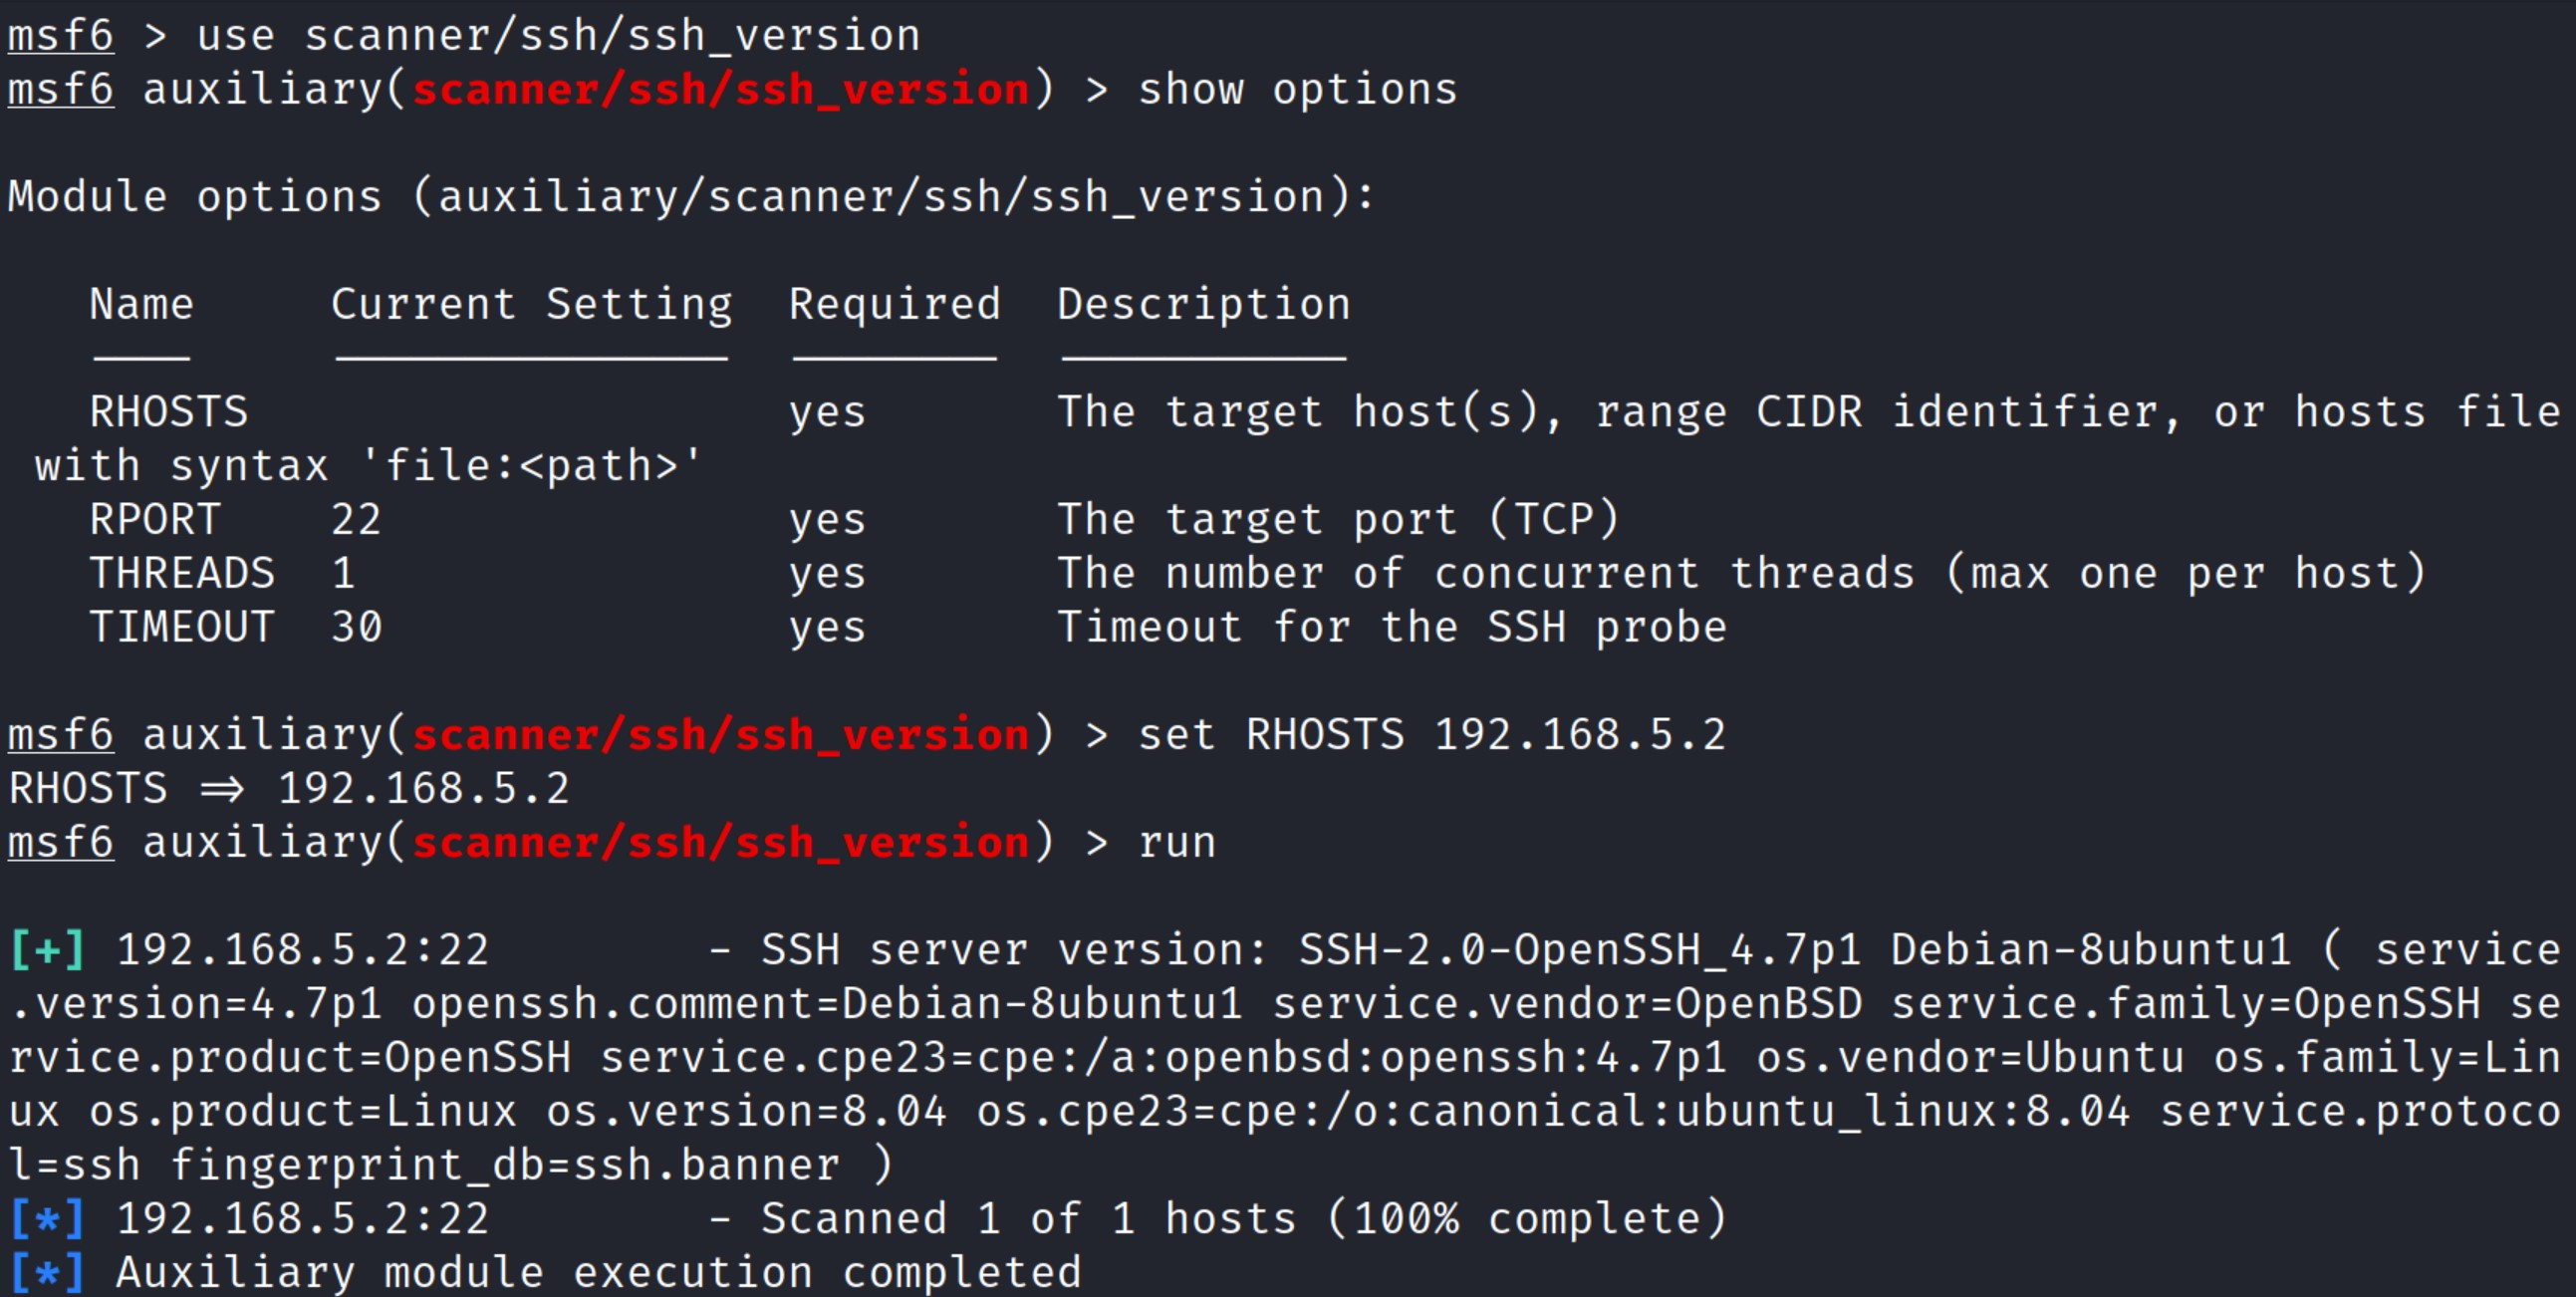
\includegraphics[width=\textwidth]{../drawable/exercise_1_screenshots/es1-ssh.jpg}
	\caption{Scanning the \texttt{SSH} version.}
	\label{fig:ex1:ssh}
\end{figure}

On first sight, it looks an innocent OpenSSH server running on top of a very old Ubuntu version. We can try the good old-fashioned way and mount a brute force attack with a dictionary file to see whether we can take over the machine without resorting to other exploits. We load the following module:

\begin{lstlisting}
use auxiliary/scanner/ssh/ssh_login
\end{lstlisting}

First, we \hltexttt{set} the \texttt{RHOSTS} variable as usual, but this time we also employ a file, called \texttt{passwords.txt} and saved in the home directory of Kali, and we \hltexttt{set} it against the \texttt{USERPASS\_FILE} variable. We can inspect the file on a separate shell:

\begin{lstlisting}
---(kali@kali)-[~]
--$ cat passwords.txt 

user password
msfadmin msfadmin
user user
root user
root password
\end{lstlisting}

For the purposes of this exercise, we inserted a handful of passwords just to show the mechanism of the module. Real life userpass files contain thousands of thousands of username and password combinations. Once the module has been executed, we should have obtained two shell logins. Figure \ref{fig:ex1:brutessh} shows the output of the module.

\begin{figure}[htbp]
	\centering
	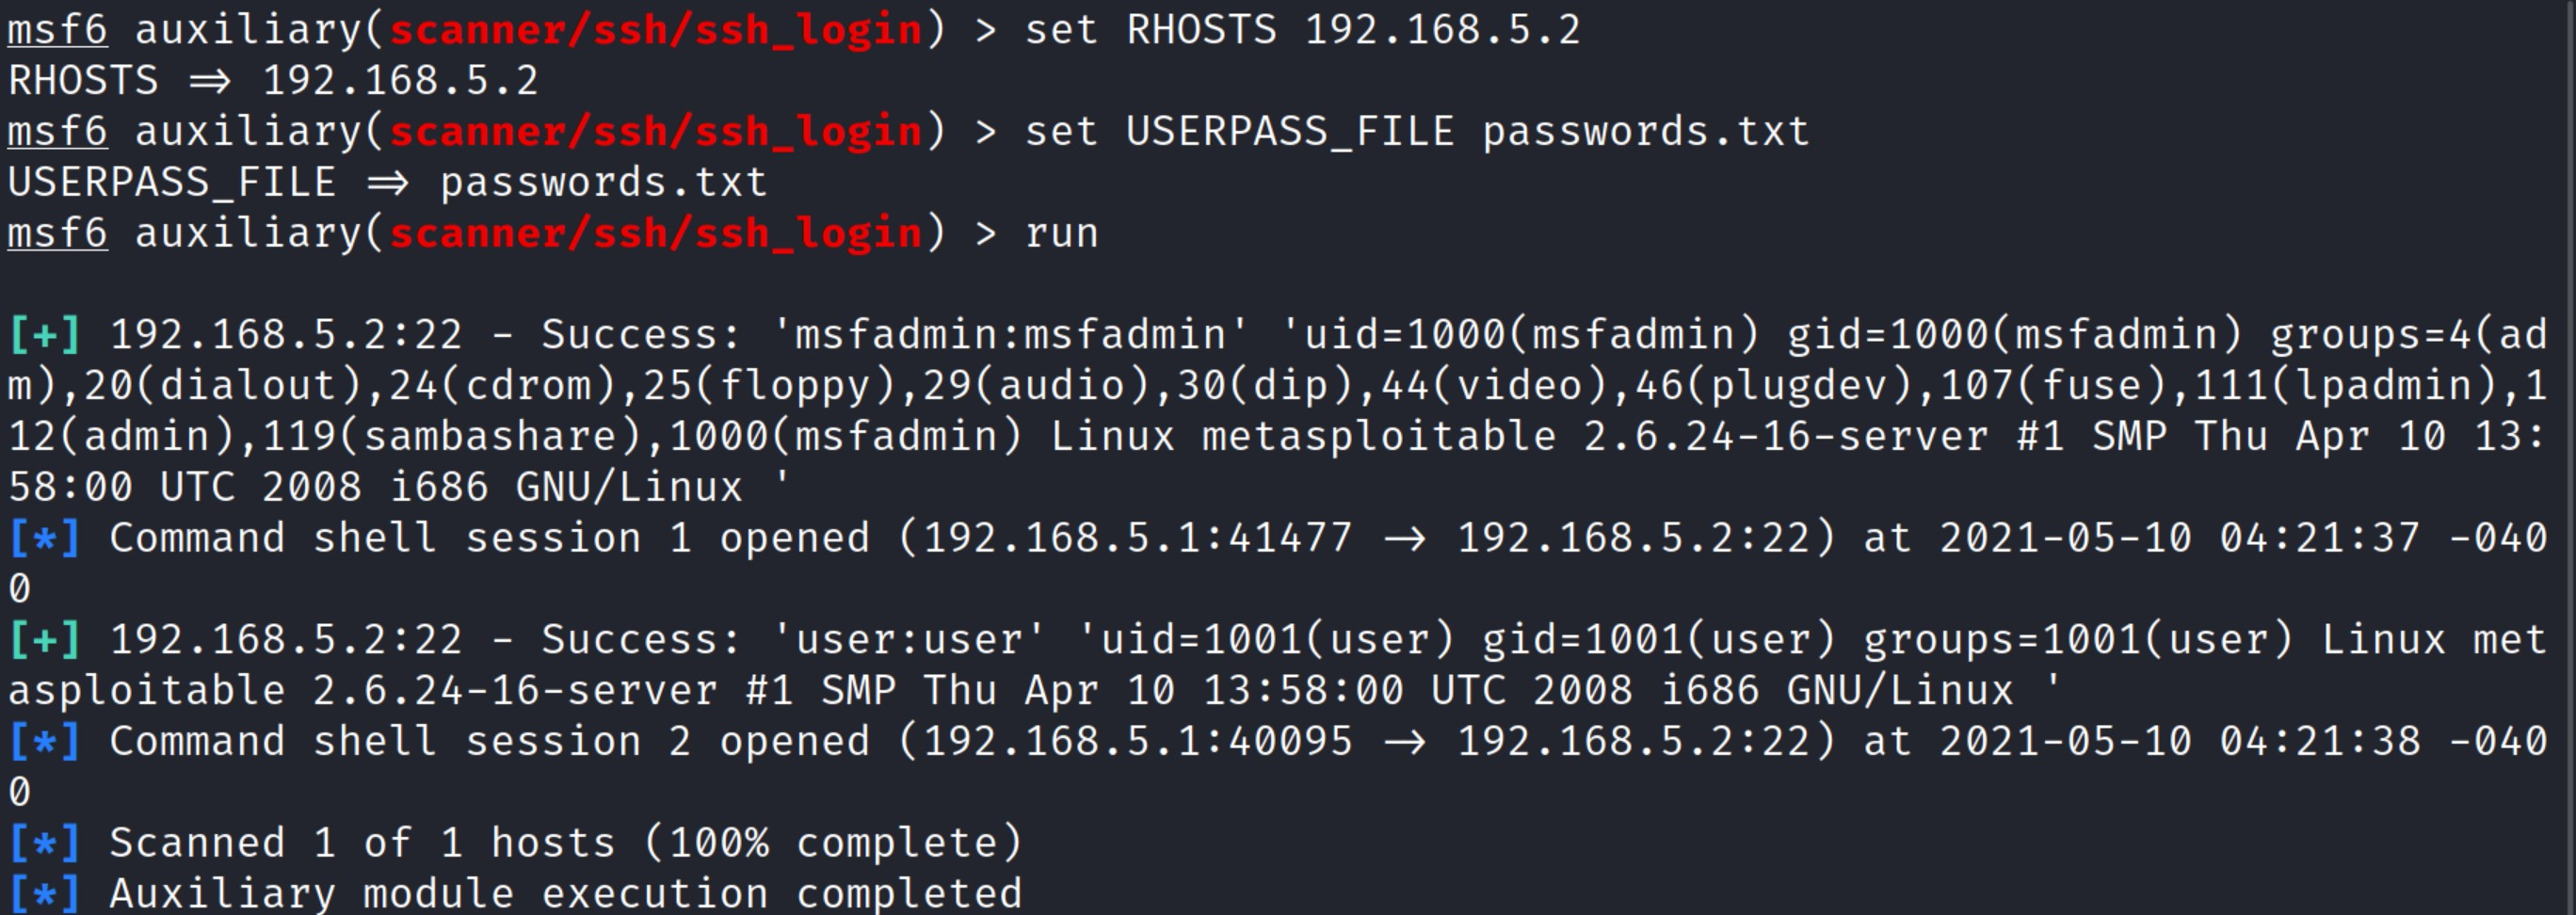
\includegraphics[width=\textwidth]{../drawable/exercise_1_screenshots/es1-brutessh.jpg}
	\caption{Taking over the \texttt{SSH} webserver with an userpass file.}
	\label{fig:ex1:brutessh}
\end{figure}

This time, we intentionally inserted two valid username and password combinations in the \texttt{passwords.txt} file. One of them (\texttt{msfadmin}, \texttt{msfadmin}) opened a full, root-privileged shell. The other one (\texttt{user}, \texttt{user}) opened a regular one. In fact, we can derive that from Figure \ref{fig:ex1:brutessh}, in which the first username/password hit shows \texttt{gid=1000(msfadmin)}, while the second one shows \texttt{gid=1001(user)}.

This resulted in two open connections. We can check the active sessions with the \hltexttt{\mbox{sessions}} command. Figure \ref{fig:ex1:sshsessions} shows the output of the command.

\begin{figure}[htbp]
	\centering
	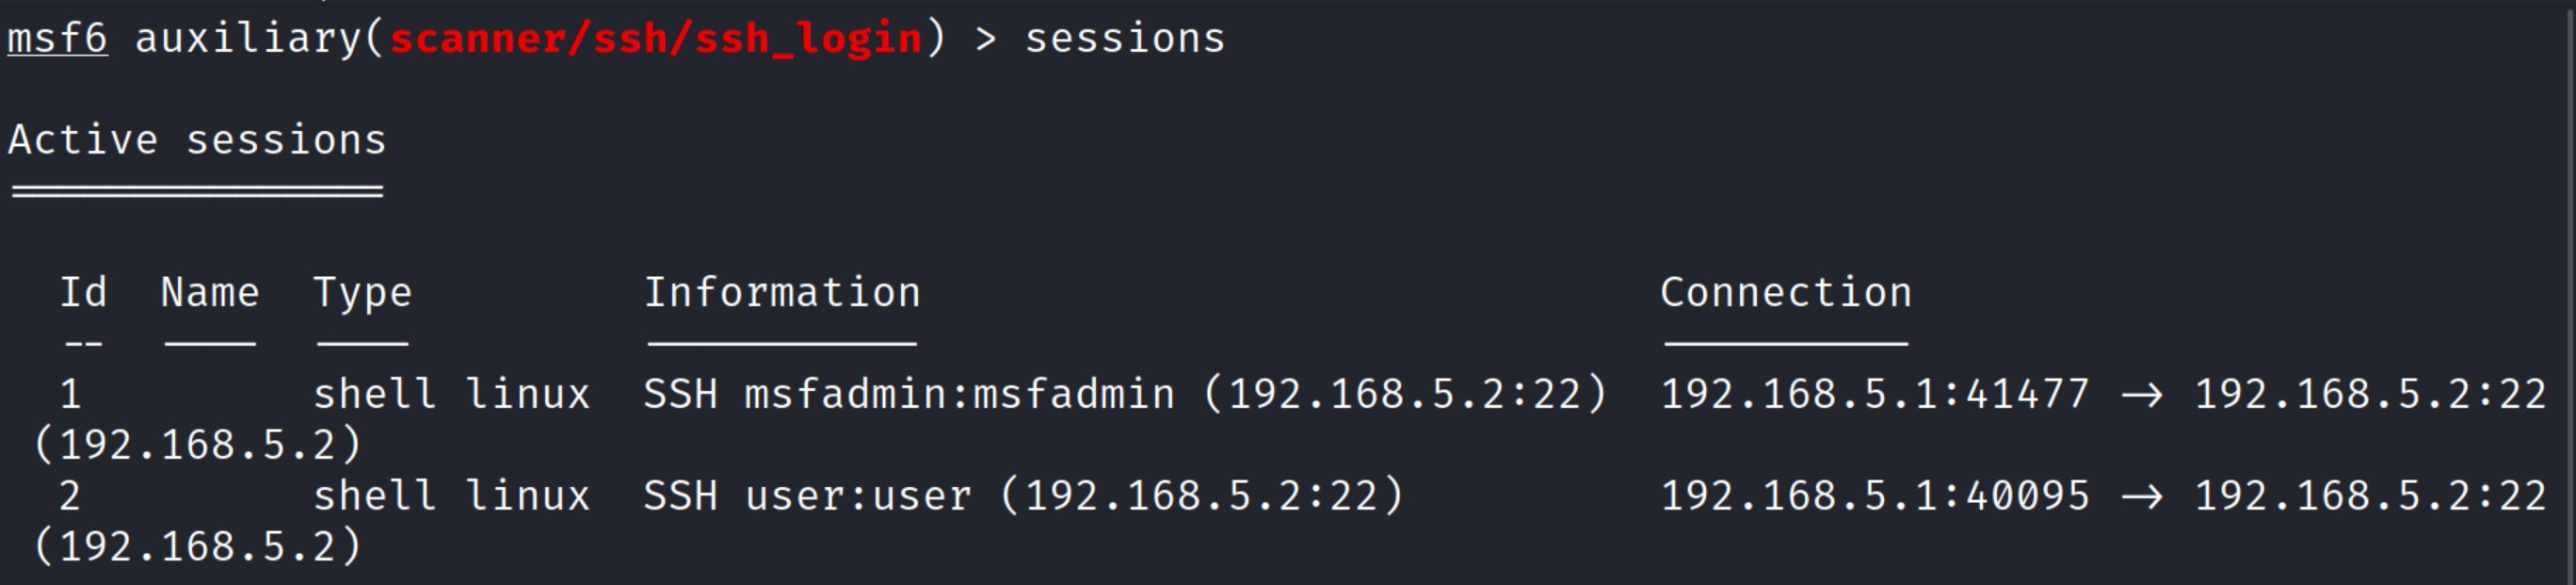
\includegraphics[width=\textwidth]{../drawable/exercise_1_screenshots/es1-sshsessions.jpg}
	\caption{The active sessions.}
	\label{fig:ex1:sshsessions}
\end{figure}

\subsection{HTTP scanning}
The amount of modules is vast. We conclude this exercise by checking the running version of a web server and listing its available directories. The following modules come into play:

\begin{lstlisting}
use auxiliary/scanner/http/http_version
use auxiliary/scanner/http/dir_scanner
\end{lstlisting}

Both modules require setting the \texttt{RHOSTS} variable to a corresponding target. We will just target the Metasploitable machine (bound on the \texttt{.2} IP address) as the XP one is not interesting in this case and has no open web server. 

\begin{figure}[htbp]
	\centering
	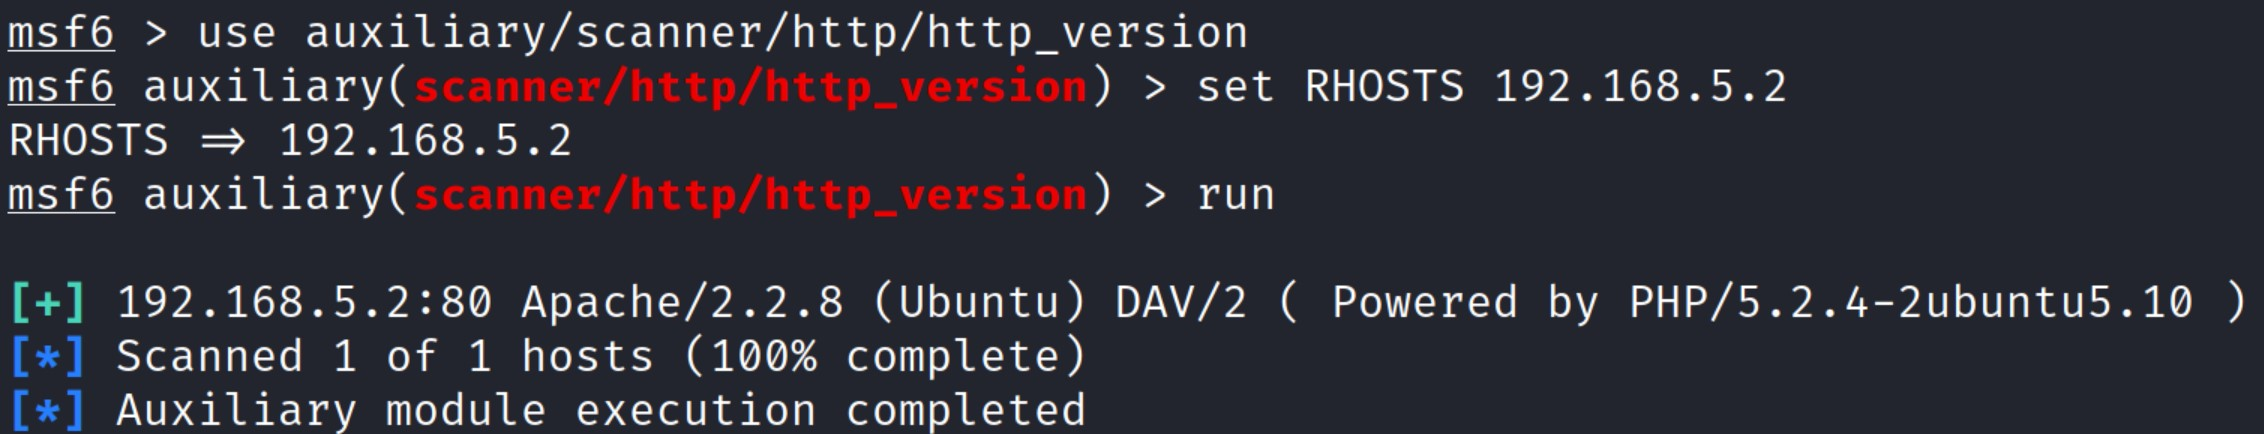
\includegraphics[width=\textwidth]{../drawable/exercise_1_screenshots/es1-http.jpg}
	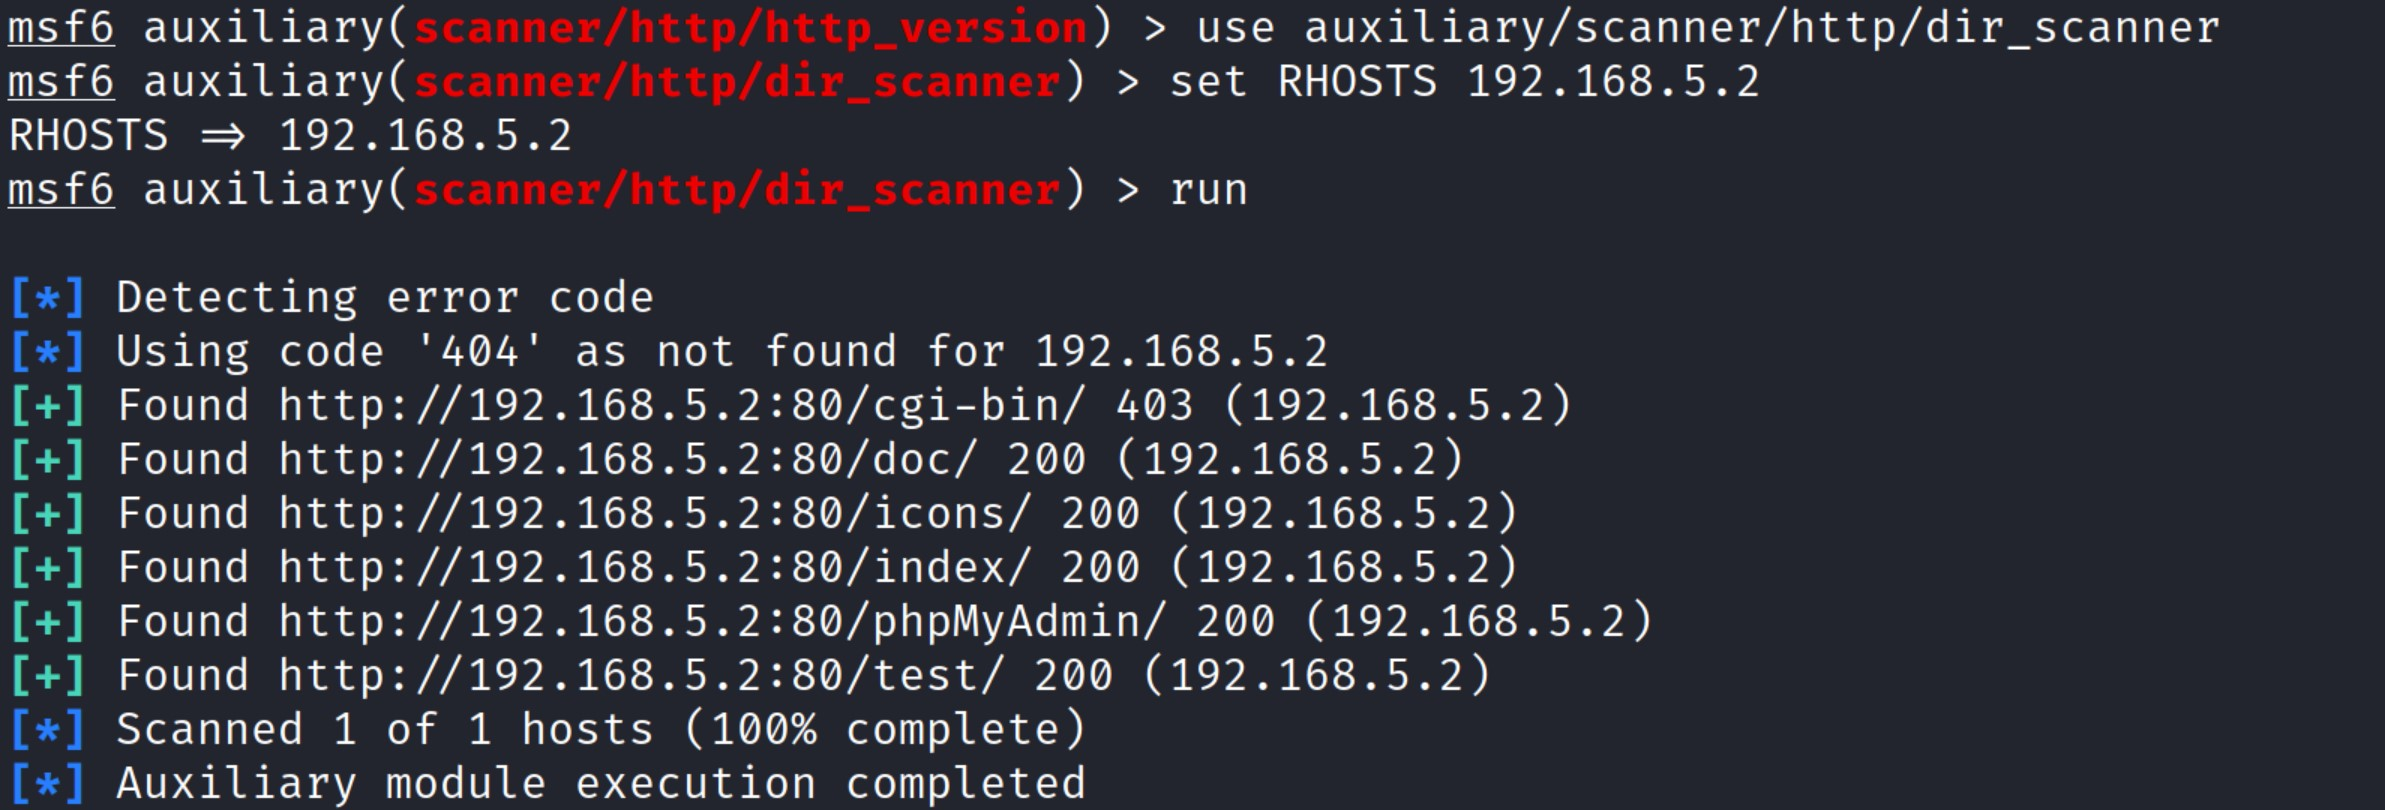
\includegraphics[width=\textwidth]{../drawable/exercise_1_screenshots/es1-httpdir.jpg}
	\caption{Scanning the HTTP version of a webserver and open directories}
	\label{fig:ex1:http}
\end{figure}

Figure \ref{fig:ex1:http} shows the output of both commands. We can observe how in the first case, we have an Apache web server running on top of a very insecure \texttt{PHP 5.2.4}, open on port \texttt{80}. This will be a very tasty target later on. To add insult to injury, a lot of directories are left exposed on the server, including the \texttt{phpMyAdmin} folder.

During the scan, it may be noticed that the scanner isn't exactly as quick as we would expect. This is because Metasploit allows customization of the number of concurrent threads (and therefore open connections) allowed during a scan. We can fix this by setting the \texttt{THREADS} variable. A value such as 50 is perfectly reasonable in a Linux environment such as ours. 

If we were,for example to launch a scan on the DISI website and its subnet (\texttt{disi.unitn.it/24}), we could see the sheer amount of tracked webservers and imagine how long it would take to scan all of them with a single thread. Figure \ref{fig:ex1:http-disi} shows a small snippet of an ongoing scan against that subnet.

\begin{figure}[htbp]
	\centering
	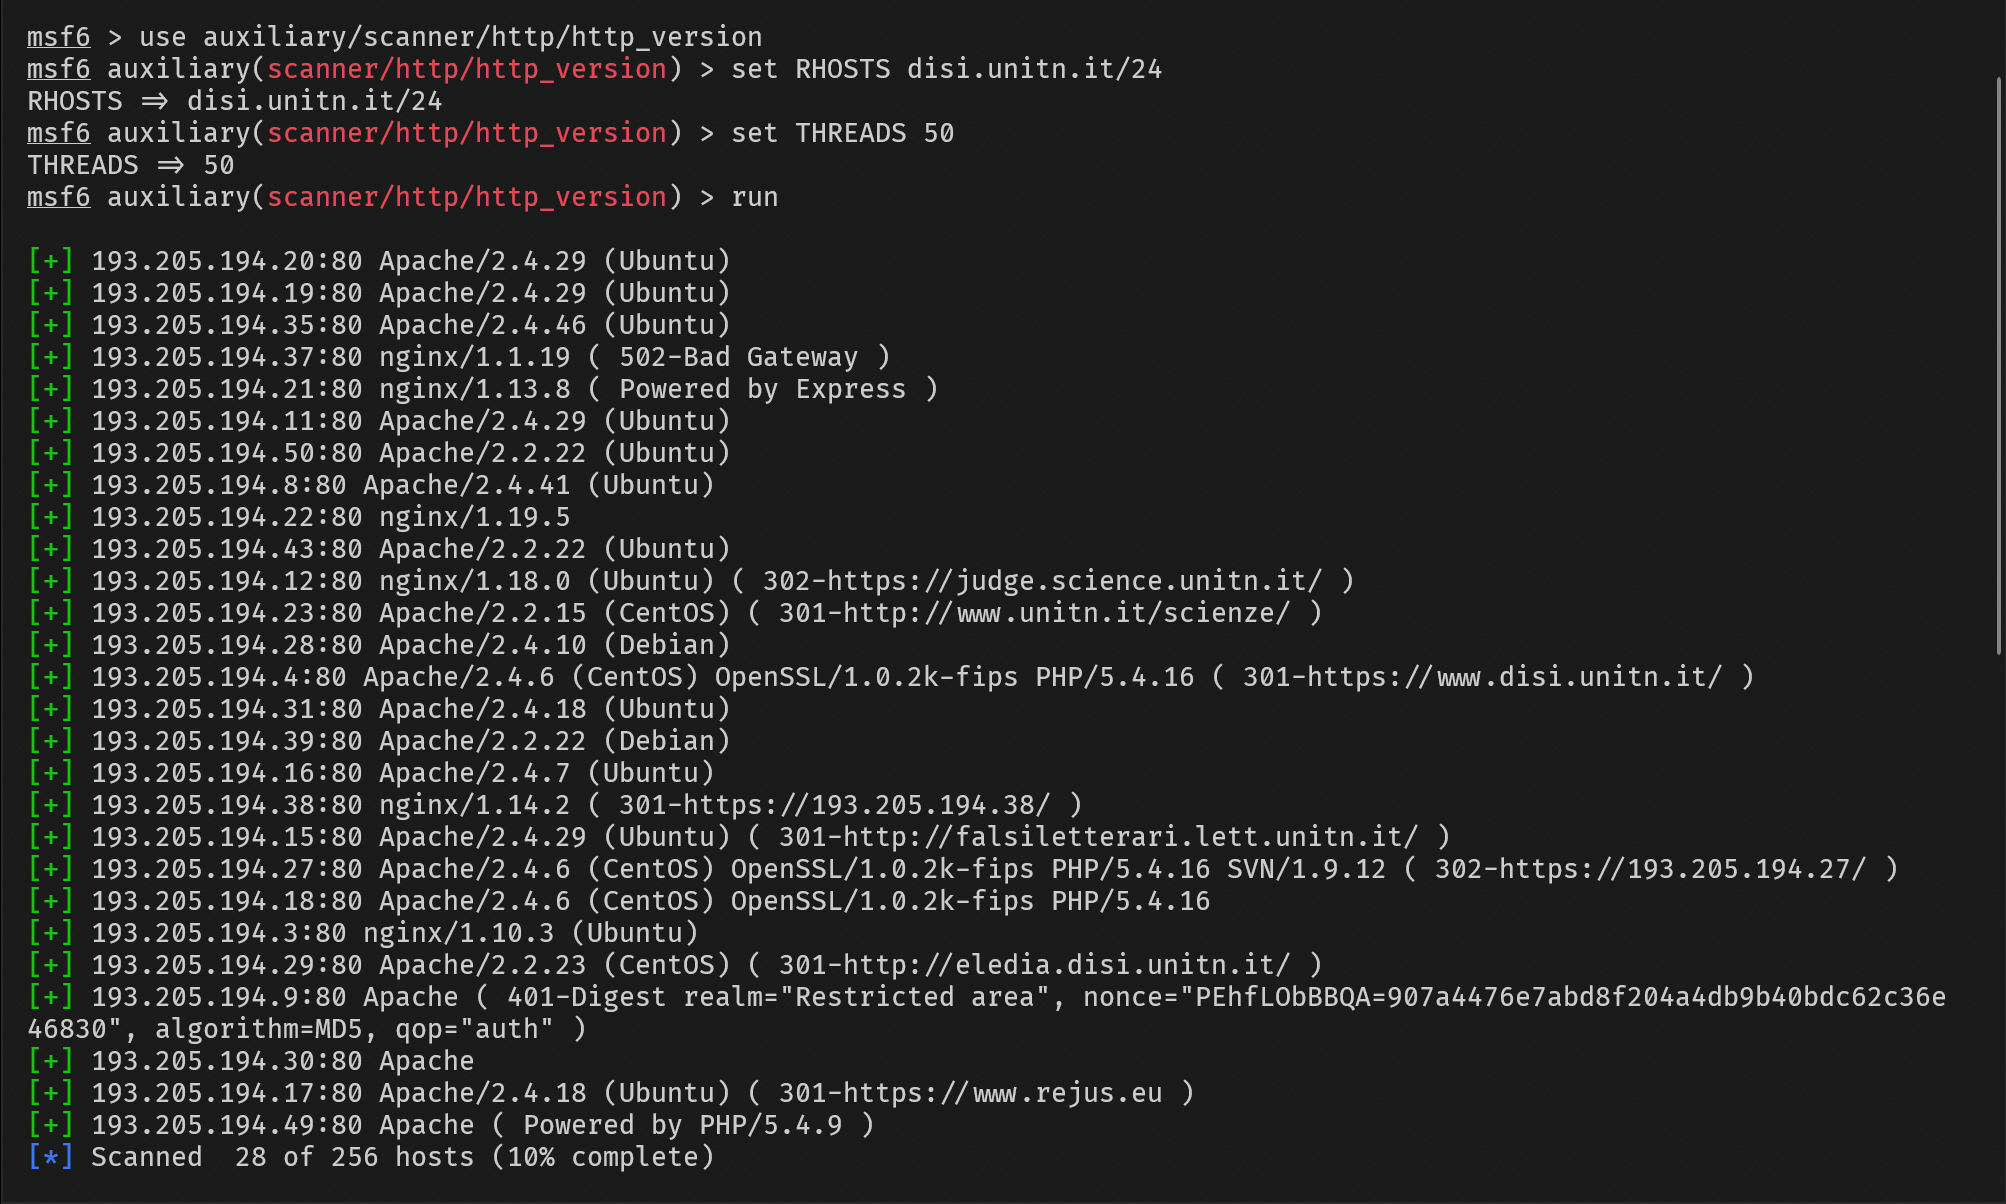
\includegraphics[width=0.85\textwidth]{../drawable/exercise_1_screenshots/es1-http-disi.png}
	\caption{Scanning the HTTP versions of the \texttt{disi.unitn.it} subnet}
	\label{fig:ex1:http-disi}
\end{figure}

This concludes the first exercise. We are now ready for a full fledged exploit against a slightly more advanced target.

\clearpage